\section{CHERI}\label{chap:bg:sec:cheri}
% Concept of a capability
In CHERI, addresses/pointers are replaced with capabilities: unforgeable tokens that provide \emph{specific kinds of access} to an \emph{address} within a \emph{range of memory}.
The above statement is enough to understand what capabilities contain\footnote{This is a slight simplification. For the purposes of vector memory accesses the \emph{otype} of a capability can be ignored, as any type other than \code{UNSEALED} cannot be dereferenced anyway.}:
\begin{itemize}
    \item Permission bits, to restrict access
    \item The \emph{cursor}, i.e. the address it currently points to
    \item The \emph{bounds}, i.e. the range of addresses this capability could point to
\end{itemize}
A great deal of work has gone into compressing capabilities down into a reasonable size (see~\cite{woodruffCHERIConcentratePractical2019}, \cref{cheri:compressedcap}), and using the magic of floating-point all of this data has been reduced to just 2x the architectural register size.
For example, on 64-bit RISC-V a standard capability is 128-bits long.
The rest of this dissertation assumes capabilities are 128-bits long for simplicity.

\begin{figure}[b]
    \centering
    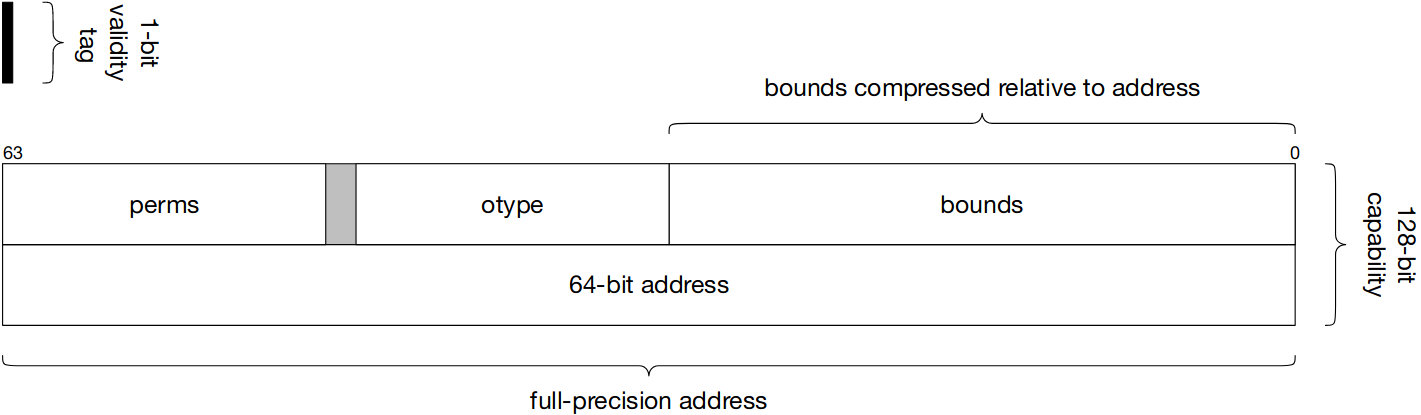
\includegraphics[width=0.8\textwidth]{./figures/cheri_compressed_cap.png}
    \caption{128-bit compressed capability representation --- from~\cite{TR-941}}\label{cheri:compressedcap}
\end{figure}

A CHERI implementation has to enforce three security properties about its capabilities\cite[Section~1.2.1]{TR-951}:
\begin{itemize}
    \item Provenance --- Capabilities must always be derived from valid manipulations of other capabilities.
    \item Integrity --- Corrupted capabilities cannot be dereferenced.
    \item Monotonicity --- Capabilities cannot increase their rights.
\end{itemize}

Integrity is enforced by tagging registers and memory.
Every 128-bit register and aligned 128-bit region of memory has an associated tag bit, which denotes if its data encodes a valid capability\footnote{This has the side-effect that capabilities must be 128-bit aligned in memory.}.
If any non-capability data is written to any part of the region the tag bit is zeroed out.
Instructions that perform memory accesses can only do so if the provided capability has a valid tag bit.
As above, significant work has gone into the implementation to reduce the DRAM overhead of this method (see~\cite{joannouEfficientTaggedMemory2017}).

\pagebreak
Provenance and Monotonicity are enforced by all instructions that manipulate capabilities.
If an implementation detects a violation of either property, it will zero out the tag bit and rely on Integrity enforcement to ensure it is not dereferenced.
Some CHERI-enabled architectures, such as CHERI-RISC-V, also raise a synchronous exception when this occurs.

\subsection{CHERI-RISC-V ISA}
The Cambridge Computer Lab's TR-951 report\cite{TR-951} describes the latest version of the CHERI architecture (CHERI ISAv8) and proposes applications to MIPS, x86-64, and RISC-V.
CHERI-RISC-V is a mostly straightforward set of additions to basic RISC-V ISAs.
It adds thirty-two general-purpose capability registers, thirty-two Special Capability Registers (SCRs), and many new instructions.

The new general-purpose capability registers are each of size \code{CLEN = 2 * XLEN} plus a tag bit.
These registers store compressed capabilities.
While there is always a logical distinction between the pre-existing \emph{integer} registers \code{x0-x31} and the \emph{capability} registers \code{cx0-cx31}, the architecture may store them in a Split or Merged register file.\label{chap:bg:subsec:cherimergedreg}
A Split register file stores the integer registers separately from capability registers, so programs can manipulate them independently.
A Merged register file stores thirty-two registers of length \code{CLEN}, using the full width for the capability registers, and aliases the integer registers to the bottom \code{XLEN} bits.
Under a merged register file, writing to an integer register makes the capability counterpart invalid, so programs have to be more careful with register usage.
% \todomark{diagram for split/merged register file?}

Many of the new SCRs are intended to support the privileged ISA extensions for e.g. hypervisors or operating systems.
The emulator doesn't use these, so their SCRs are not listed here, but there are two highly relevant SCRs for all modes: the Program Counter Capability and the Default Data Capability.

The PCC replaces the program counter and adds more metadata, ensuring instruction fetches have the same security properties as normal loads and stores.
The DDC is used to sandbox integer addressing modes.
CHERI-RISC-V includes new instructions which use integer addressing, and allows legacy (i.e. integer addressed) code to function on CHERI systems without recompiling for CHERI-RISC-V.
These instructions all use integer addresses relative to the DDC, and the DDC controls the permissions those instructions have.

\subsection{Instruction changes}\label{cheri_instructions}
TR-951\cite[Chapter~8]{TR-951} specifies a suite of new instructions, as well as a set of modifications to pre-existing instructions.
Many of the new instructions are unrelated to pre-existing instructions, and implement capability-specific operations like accessing fields of capability registers.
The most relevant new instructions for our case are the various loads/stores.

\pagebreak
CHERI-RISC-V adds new instructions for loading integer and capability data, either via capabilities or using integer addressing through the DDC (\cref{tab:new_cheri_instrs}).
These instructions are intended for hybrid-capability code (see \cref{cheri_purecap_hybrid},~\cite[p151]{TR-951}), so are more limited and don't support immediate offsets.
The behaviour of basic RISC-V load/store opcodes changes to either use capabilities as memory references or use integer addressing via the DDC, depending on the encoding mode.
If any instruction tries to dereference an invalid capability, it raises a synchronous exception.

\begin{table}[t]
    \centering
    \begin{tabular}{lccl}
    \toprule
        Name & Direction & Data type & Address calculation \\
        \midrule
        L[BHWD][U].CAP & Load & Integer & via capability register \\
        L[BHWD][U].DDC & Load & Integer & via DDC \\
        LC.CAP & Load & Capability & via capability register \\
        LC.DDC & Load & Capability & via DDC \\ 
        S[BHWD].CAP & Store & Integer & via capability register \\
        S[BHWD].DDC & Store & Integer & via DDC \\
        SC.CAP & Store & Capability & via capability register \\
        SC.DDC & Store & Capability & via DDC \\ 
    \bottomrule
    \end{tabular}
    \caption{New CHERI load/store instructions}
    \label{tab:new_cheri_instrs}
\end{table}
\begin{table}[t]
    \centering
    \begin{tabular}{lccc}
    \toprule
        Name & Direction & Data type & \multicolumn{1}{c}{Address calculation} \\
        &&& (Capability/Integer mode) \\
        \midrule
        {[C]}LC\parnote{Replaces RV128 LQ} & Load & Capability & via capability/DDC \\
        {[C]}SC\parnote{Replaces RV128 SQ} & Store & Capability & via capability/DDC \\
        \midrule
        L[BWHD][U] & Load & Integer & via capability/DDC \\
        S[BWHD] & Store & Integer & via capability/DDC \\
        FL[WDQ] & Load & Float & via capability/DDC \\
        FS[WDQ] & Store & Float & via capability/DDC \\
        LR & Load & Integer & via capability/DDC \\
        SC & Store & Integer & via capability/DDC \\
        AMO\parnote{All atomic memory operations} & --- & Integer & via capability/DDC \\
    \bottomrule
    \end{tabular}
    \parnotes
    \caption{Preexisting RISC-V load/store instructions modified by CHERI-RISC-V}
    \label{tab:legacy_cheri_instrs}
\end{table}

\subsection{Capability and Integer encoding mode\label{chap:bg:subsec:cheriencodingmode}}
CHERI-RISC-V specifies two encoding modes, selected using a flag in the PCC \code{flags} field.
\emph{Capability mode} modifies the behaviour of pre-existing instructions to take address operands as capabilities.
This makes the basic load/store instruction behaviour exactly equivalent to newly introduced counterparts: e.g. \code{L[BWHD][U] == L[BWHD][U].CAP}.
The DDC may still be used in this mode via the new instructions e.g. \code{S[BWHD].DDC}.

\pagebreak
\emph{Integer mode} seeks to emulate a standard CHERI-less RISC-V architecture as much as possible.
All pre-existing RISC-V memory access instructions take address operands as integers, which are dereferenced relative to the DDC\footnote{Of course, the DDC must be valid when it is used in this mode, and all bounds checks etc. must still pass.}.
This makes the basic load/store instruction behaviour exactly equivalent to newly introduced counterparts: e.g. \code{L[BWHD][U] == L[BWHD][U].DDC}.
The new instructions may still be used to dereference and inspect capability registers, but all other instructions access registers in an integer context i.e. ignoring the upper bits and tag from merged register files.

\subsection{Pure-capability and Hybrid compilation modes}\label{cheri_purecap_hybrid}
CHERI-Clang\footnote{\url{https://www.cl.cam.ac.uk/research/security/ctsrd/cheri/cheri-llvm.html}}, the main CHERI-enabled compiler, supports two ways to compile CHERI-RISC-V which map to the different encoding modes.

\emph{Pure-capability} mode treats all pointers as capabilities, and emits pre-existing RISC-V instructions that expect to be run in capability mode\footnote{This wasn't derived from documentation, but instead from manual inspection of emitted code.}.

\emph{Hybrid} mode treats pointers as integer addresses, dereferenced relative to the DDC, unless they are annotated with \code{\_\_capability}.
This mode emits pre-existing RISC-V instructions that take integer operands, and uses capabilities through the new instructions.
All capabilities in hybrid mode are created manually by the program by copying and shrinking the DDC.

Hybrid mode allows programs to be gradually ported to CHERI, making it very easy to adopt on legacy/large codebases.
Any extensions to the model (e.g. CHERI-RVV) should try and retain this property.

\subsection{Capability relocations\label{chap:bg:subsec:cherirelocs}}
\emph{Summarizes~\cite[Section~4.4, Appendix C]{TR-949}}

Binary applications compiled in pure-capability mode require some ``global'' capabilities to exist at startup, e.g. the capability which points to the \code{main()} function.
It would be a security risk to synthesize these capabilities from thin air, or to allow the binary file itself to contain tag bits.

Instead, CHERI ELF binaries contain a set of requested ``relocations'' (the \code{\_\_cap\_relocs} section) which instruct the runtime environment to create capabilities with specific permissions and bounds in specific places.
This process uses the normal CHERI capability instructions, so any invalid requests will cause a program crash, maintaining security.
Further complexity is introduced with dynamic linking, and in the future these relocations may change format, both described in TR-949\cite{TR-949}, but the above description is sufficient to understand the rest of this paper.

% \subsection{Instruction reference}
% \todomark{TR-951 contains a complete reference of all added instructions in section blah, and notes legacy instructions modified by capability mode in section blah. Reproduce short list? Do so in appendix?}